
%(BEGIN_QUESTION)
% Copyright 2011, Tony R. Kuphaldt, released under the Creative Commons Attribution License (v 1.0)
% This means you may do almost anything with this work of mine, so long as you give me proper credit

A team of technicians has built this gas compressor system, and are nearly ready to start it up.  The system provides over-current protection for the compressor's drive motor using fuses, while a data acquisition unit (DAQ) monitors compressor discharge pressure and vibration.  

Just days before the planned start-up, you happen to perform an inspection of their work.  You see 480 VAC (three-phase) power routed to the compressor's drive motor through fuses in the first enclosure.  You also see two sensors at the compressor -- a high-pressure alarm switch (24 VDC discrete on/off signal) and a vibration probe (outputting millivolt signals proportional to compressor vibration) -- connected to a data acquisition unit located at the first enclosure.  All wiring is in the form of individual conductors, with the exception of the multi-conductor RS-232 cable connecting the DAQ to the operator's computer display:

$$\includegraphics[width=15.5cm]{i02400x01.eps}$$

Your answer should consist of two parts: (1) identify any potential problems you see in the measurement wiring, and (2) explain how you would modify this system to improve it.

\underbar{file i02400}
%(END_QUESTION)





%(BEGIN_ANSWER)

Half-credit for identifying problem, and half-credit for suggesting a practical solution.

\vskip 10pt

The problem is the near-certainty of AC power line noise coupling onto the millivolt vibration probe signal wires as they run parallel to the 480 VAC power conductors in the conduit.  

Multiple options exist to avoid noise coupling on to the vibration probe signal wires, each one of them valid:

\begin{itemize}
\item{} Install a separate conduit just for signal wires
\item{} Re-locate the DAQ to the right-hand enclosure, so RS-232 cabling runs parallel to the power wiring rather than analog signal wires
\item{} Use twisted-pair, shielded wire for the analog signals rather than individual wires, to protect the analog signal from picking up interference from the AC power wires
\end{itemize}

%(END_ANSWER)





%(BEGIN_NOTES)

{\bf This question is intended for exams only and not worksheets!}.

%(END_NOTES)


